\section{Neutron Detection}
\subsection{General Remarks}
\begin{itemize}
    \item Neutrons are charge-neutral particles; they can only interact via the strong force and ionize via secondary reactions.
    \item Most neutron detectors consist of a material that converts neutrons into charged particles within a conventional detector.
    \item There are 2 classes of interactions:
    \begin{enumerate}
        \item Slow neutrons (thermal and epithermal), E $<$ 1 keV:\\
        (n,$\gamma$), (n,p), (n,$\alpha$), (n,f)
        \item Fast neutrons, E $>$ 1 keV:\\
        (n,n), (n,n'), (n,xn), (n,xpn), (n,f)
    \end{enumerate}
\end{itemize}
\subsection{Slow Neutron Detection}
\subsubsection{Commonly Used Neutron Reactions}
\begin{itemize}
    \item Commonly used reactions include:
    \begin{itemize}
        \item (n,p):
        \begin{itemize}
            \item[] n $+$ $^3$He $\rightarrow$ p $+$ $^3$H, Q $=$ 0.765 MeV
        \end{itemize}
        \item (n,$\alpha$):
        \begin{itemize}
            \item[] n $+$ $^6$Li $\rightarrow$ $^4$He $+$ $^3$H, Q $=$ 4.78 MeV
            \item[] n $+$ $^{10}$B $\rightarrow$ $^{4}$He $+$ $^7$Li*, Q $=$ 2.31 MeV (94\%)
            \item[] n $+$ $^{10}$B $\rightarrow$ $^{4}$He $+$ $^7$Li, Q $=$ 2.79 MeV (6\%)
        \end{itemize}
        \item (n,$\gamma$): $\sigma\propto1/v$
        \begin{itemize}
            \item[] n $+$ $^{113}$Cd $\rightarrow$ $^{114}$Cd $+$ $\gamma$, Q $\sim$ 8 MeV
            \item[] n $+$ $^{157}$Gd $\rightarrow$ $^{158}$Gd $+$ $\gamma$, Q $\sim$ 8 MeV
        \end{itemize}
        \item (n,f):
        \begin{itemize}
            \item[] n $+$ $^{235}$U $\rightarrow$ fission fragments, Q $\sim$ 200 MeV
        \end{itemize}
    \end{itemize}
\end{itemize}

\subsubsection{The He-3 Proportional Counter}
\begin{itemize}
    \item n $+$ $^3$He $\rightarrow$ p $+$ $^3$H, Q $=$ 764 keV
    \item Assuming E$_n\ll$ Q, with momentum conservation, E$_p=\frac{m_t}{m_p+m_t}$Q $=$ 573 keV, E$_t=\frac{m_p}{m_p+m_t}$Q $=$ 191 keV.
    \item The wall effect, as shown in figure~\ref{fig:He3_wall_effect}, occurs as the proton or triton may escape without detection. The wall effect depends on the tube dimensions and gas pressure. Methods to decrease the wall effect include:
    \begin{itemize}
        \item Building a counter with a diameter as large as possible
        \item Reducing the range of charged particles in $^3$He ($\sim$mm) by increasing gas pressure
        \item Reducing the range of charged particles by adding a small amount of a heavier gas
    \end{itemize} 
\end{itemize}
\begin{figure}[ht]
    \centering
    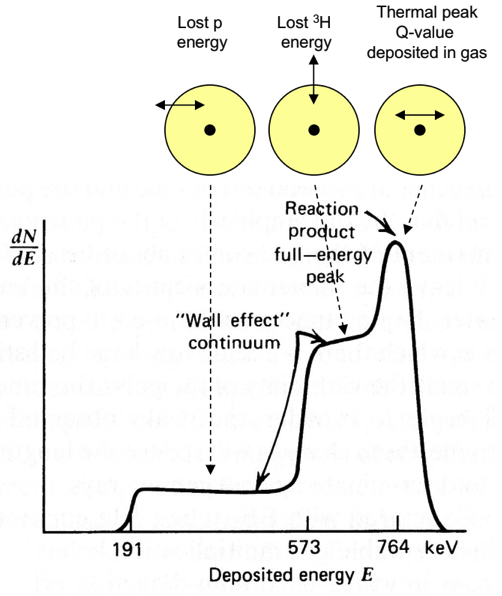
\includegraphics[width=0.4\textwidth]{images/He3_wall_effect.png}
    \caption{Wall effect in the $^3$He proportional counter.}
    \label{fig:He3_wall_effect}
\end{figure}
\subsubsection{The BF3 Slow Neutron Detector}
\begin{figure}[ht]
    \centering
    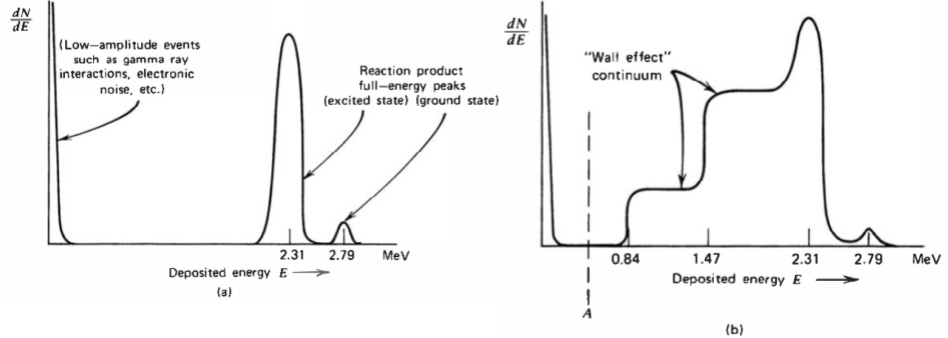
\includegraphics[width=0.8\textwidth]{images/BF3_wall_effect.png}
    \caption{The (a) ideal spectrum and (b) the wall effect in a BF$_3$ proportional tube.}
    \label{fig:BF3_wall_effect}
\end{figure}
\begin{itemize}
    \item n $+$ $^{10}$B $\rightarrow$ $^{4}$He $+$ $^7$Li*, Q $=$ 2.31 MeV (94\%)\\
          n $+$ $^{10}$B $\rightarrow$ $^{4}$He $+$ $^7$Li, Q $=$ 2.79 MeV (6\%)
    \item The BF$_3$ gas is enriched to $>$90\% $^{10}$B
    \item Operated as a proportional or GM counter
    \item To reduce the effects of recombination and negative ion formation, the gas pressure is kept below 1 atm (range of $\alpha$ $\sim$10 mm), leading to pronounced wall effect, as shown in figure~\ref{fig:BF3_wall_effect}.
    \item As in the case of the $^3$He counter, the spectrum reflects the response of the detector, $\emph{not}$ neutron energy. 
    \item BF$_3$ tubes can discriminate against low fluxes of gamma-rays; due to the low stopping power of the secondary electrons created via the interaction of gammas with the detector wall, only a small amount of energy will be deposited, leading to the low-amplitude pulses left to point A in figure~\ref{fig:BF3_wall_effect}(b).
\end{itemize}

\subsubsection{Fission Counters}
\begin{figure}[ht]
    \centering
    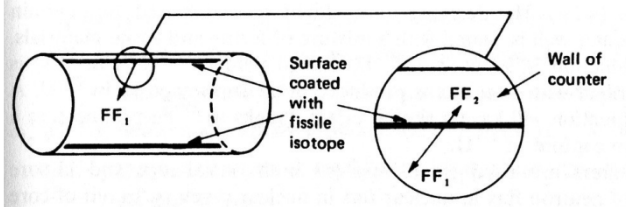
\includegraphics[width=0.4\textwidth]{images/fission_counter_config.png}
    \caption{Configuration of fission counters.}
    \label{fig:fission_counter_config}
\end{figure}
\begin{itemize}
    \item The most common form of fission detectors is an ionization chamber (or proportional counter) that has its inner surfaces coated with a fissile deposit, as shown in figure~\ref{fig:fission_counter_config}.
    \item A large amount of energy is released in each fission reaction ($\sim$200 MeV), with $\sim$160 MeV as the kinetic energy of fission fragments. Therefore, extremely low background rates can be achieved, and neutron counting can be performed with very low count rates. 
    \item Due to the non-linearities for densely ionizing particles (fission fragments), the detector pulses may not be as large as would be calculated based on simple linearity with energy, reducing discrimination capabilities.
    \item Alpha-decay of the fissile deposit creates a continuous background. 
    \item Efficiency of the counter can be increased by increasing the thickness of the deposit, but at the expense of quantitative measurement capabilities. As shown in figure~\ref{fig:fission_counter_efficiency}, while increasing thickness increases detection efficiency, the energy loss of fragments within the deposit will reduce the average fragment energy and distort the shape of the distribution. 
\end{itemize}
\begin{figure}[ht]
    \centering
    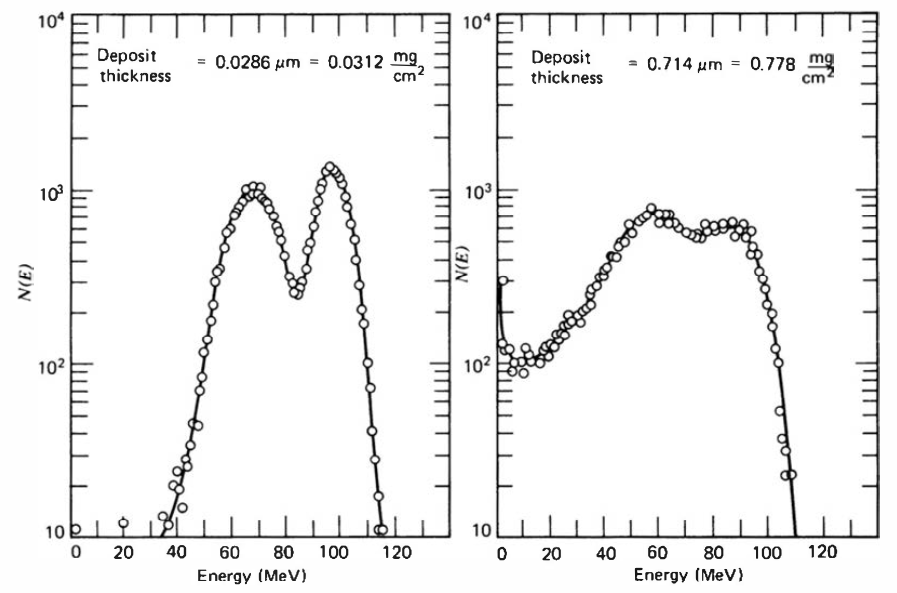
\includegraphics[width=0.6\textwidth]{images/fission_counter_efficiency.png}
    \caption{Energy spectra of fission counters with a thin layer (left) and a thicker layer (right) of fissile deposit.}
    \label{fig:fission_counter_efficiency}
\end{figure}
\subsubsection{Li-Based Scintillators}
\begin{itemize}
    \item n $+$ $^6$Li $\rightarrow$ $^4$He $+$ $^3$H, Q $=$ 4.78 MeV
    \item While there are no Li containing gas available, we have solid LiI(Eu) detectors, similar to NaI(Tl) detectors.
    \item Since the range of reaction products are shorter than dimensions of the detector, there is no wall effect; a single peak will be seen on the spectrum.
    \item The gamma rejection capabilities are inferior to gas-filled detectors; there is a continuous gamma background. (A 4.1 MeV electron will yield about the same light as the 4.78 MeV neutron induced reaction products.)
    \item $^6$Li-glass can be implemented as meters-long fibers, and is capable of fast neutron detection as well. 
    \item Liquid Li-based scintillators allows neutron-gamma pulse-shape discrimination.
\end{itemize}
\subsubsection{Elpasolites}
\begin{itemize}
    \item Dual-mode (neutron and gamma) crystalline scintillator
    \item Neutron sensitivity for thermal (capture on $^6$Li) and fast (PSD) neutrons
    \item High light yield and good proportionality for gamma spectroscopy
    \item Examples include CLYC (Cs$_2$LiYCl$_6$(Eu)) and CLLBC (Cs$_2$LiLa(Br,Cl)$_6$(Eu)) detectors
\end{itemize}

\subsection{Fast Neutron Detection}


\subsubsection{Counters Based on Moderation}


\subsubsection{Fast Neutron Scattering}


\subsubsection{The He-3 Proportional Counter}


\subsubsection{Other Fast Neutron Detectors}


\subsubsection{Pulse-Shape Discrimination}


\subsection{Miscellaneous Neutron Detectors}
\subsubsection{Nuclear Reactor Instrumentation}